% Options for packages loaded elsewhere
\PassOptionsToPackage{unicode}{hyperref}
\PassOptionsToPackage{hyphens}{url}
%
\documentclass[
]{article}
\usepackage{amsmath,amssymb}
\usepackage{lmodern}
\usepackage{iftex}
\ifPDFTeX
  \usepackage[T1]{fontenc}
  \usepackage[utf8]{inputenc}
  \usepackage{textcomp} % provide euro and other symbols
\else % if luatex or xetex
  \usepackage{unicode-math}
  \defaultfontfeatures{Scale=MatchLowercase}
  \defaultfontfeatures[\rmfamily]{Ligatures=TeX,Scale=1}
\fi
% Use upquote if available, for straight quotes in verbatim environments
\IfFileExists{upquote.sty}{\usepackage{upquote}}{}
\IfFileExists{microtype.sty}{% use microtype if available
  \usepackage[]{microtype}
  \UseMicrotypeSet[protrusion]{basicmath} % disable protrusion for tt fonts
}{}
\makeatletter
\@ifundefined{KOMAClassName}{% if non-KOMA class
  \IfFileExists{parskip.sty}{%
    \usepackage{parskip}
  }{% else
    \setlength{\parindent}{0pt}
    \setlength{\parskip}{6pt plus 2pt minus 1pt}}
}{% if KOMA class
  \KOMAoptions{parskip=half}}
\makeatother
\usepackage{xcolor}
\IfFileExists{xurl.sty}{\usepackage{xurl}}{} % add URL line breaks if available
\IfFileExists{bookmark.sty}{\usepackage{bookmark}}{\usepackage{hyperref}}
\hypersetup{
  hidelinks,
  pdfcreator={LaTeX via pandoc}}
\urlstyle{same} % disable monospaced font for URLs
\usepackage[margin=1in]{geometry}
\usepackage{longtable,booktabs,array}
\usepackage{calc} % for calculating minipage widths
% Correct order of tables after \paragraph or \subparagraph
\usepackage{etoolbox}
\makeatletter
\patchcmd\longtable{\par}{\if@noskipsec\mbox{}\fi\par}{}{}
\makeatother
% Allow footnotes in longtable head/foot
\IfFileExists{footnotehyper.sty}{\usepackage{footnotehyper}}{\usepackage{footnote}}
\makesavenoteenv{longtable}
\usepackage{graphicx}
\makeatletter
\def\maxwidth{\ifdim\Gin@nat@width>\linewidth\linewidth\else\Gin@nat@width\fi}
\def\maxheight{\ifdim\Gin@nat@height>\textheight\textheight\else\Gin@nat@height\fi}
\makeatother
% Scale images if necessary, so that they will not overflow the page
% margins by default, and it is still possible to overwrite the defaults
% using explicit options in \includegraphics[width, height, ...]{}
\setkeys{Gin}{width=\maxwidth,height=\maxheight,keepaspectratio}
% Set default figure placement to htbp
\makeatletter
\def\fps@figure{htbp}
\makeatother
\setlength{\emergencystretch}{3em} % prevent overfull lines
\providecommand{\tightlist}{%
  \setlength{\itemsep}{0pt}\setlength{\parskip}{0pt}}
\setcounter{secnumdepth}{5}
\usepackage{graphicx}
\usepackage{hyperref}
\ifLuaTeX
  \usepackage{selnolig}  % disable illegal ligatures
\fi

\author{}
\date{\vspace{-2.5em}}

\begin{document}

%! Author = Niek Scholten
%! Date = 24-10-2022

%Turn off page numbering
\pagenumbering{gobble}
\begin{center}

    \Huge{Predicting bird species from their songs using machine learning}\\
    \vspace{\baselineskip}
    \LARGE{Theme 09 - Introduction Machine Learning}\\
    \large{Research paper}\\
    \vspace{\baselineskip}

    \begin{figure}
        \centering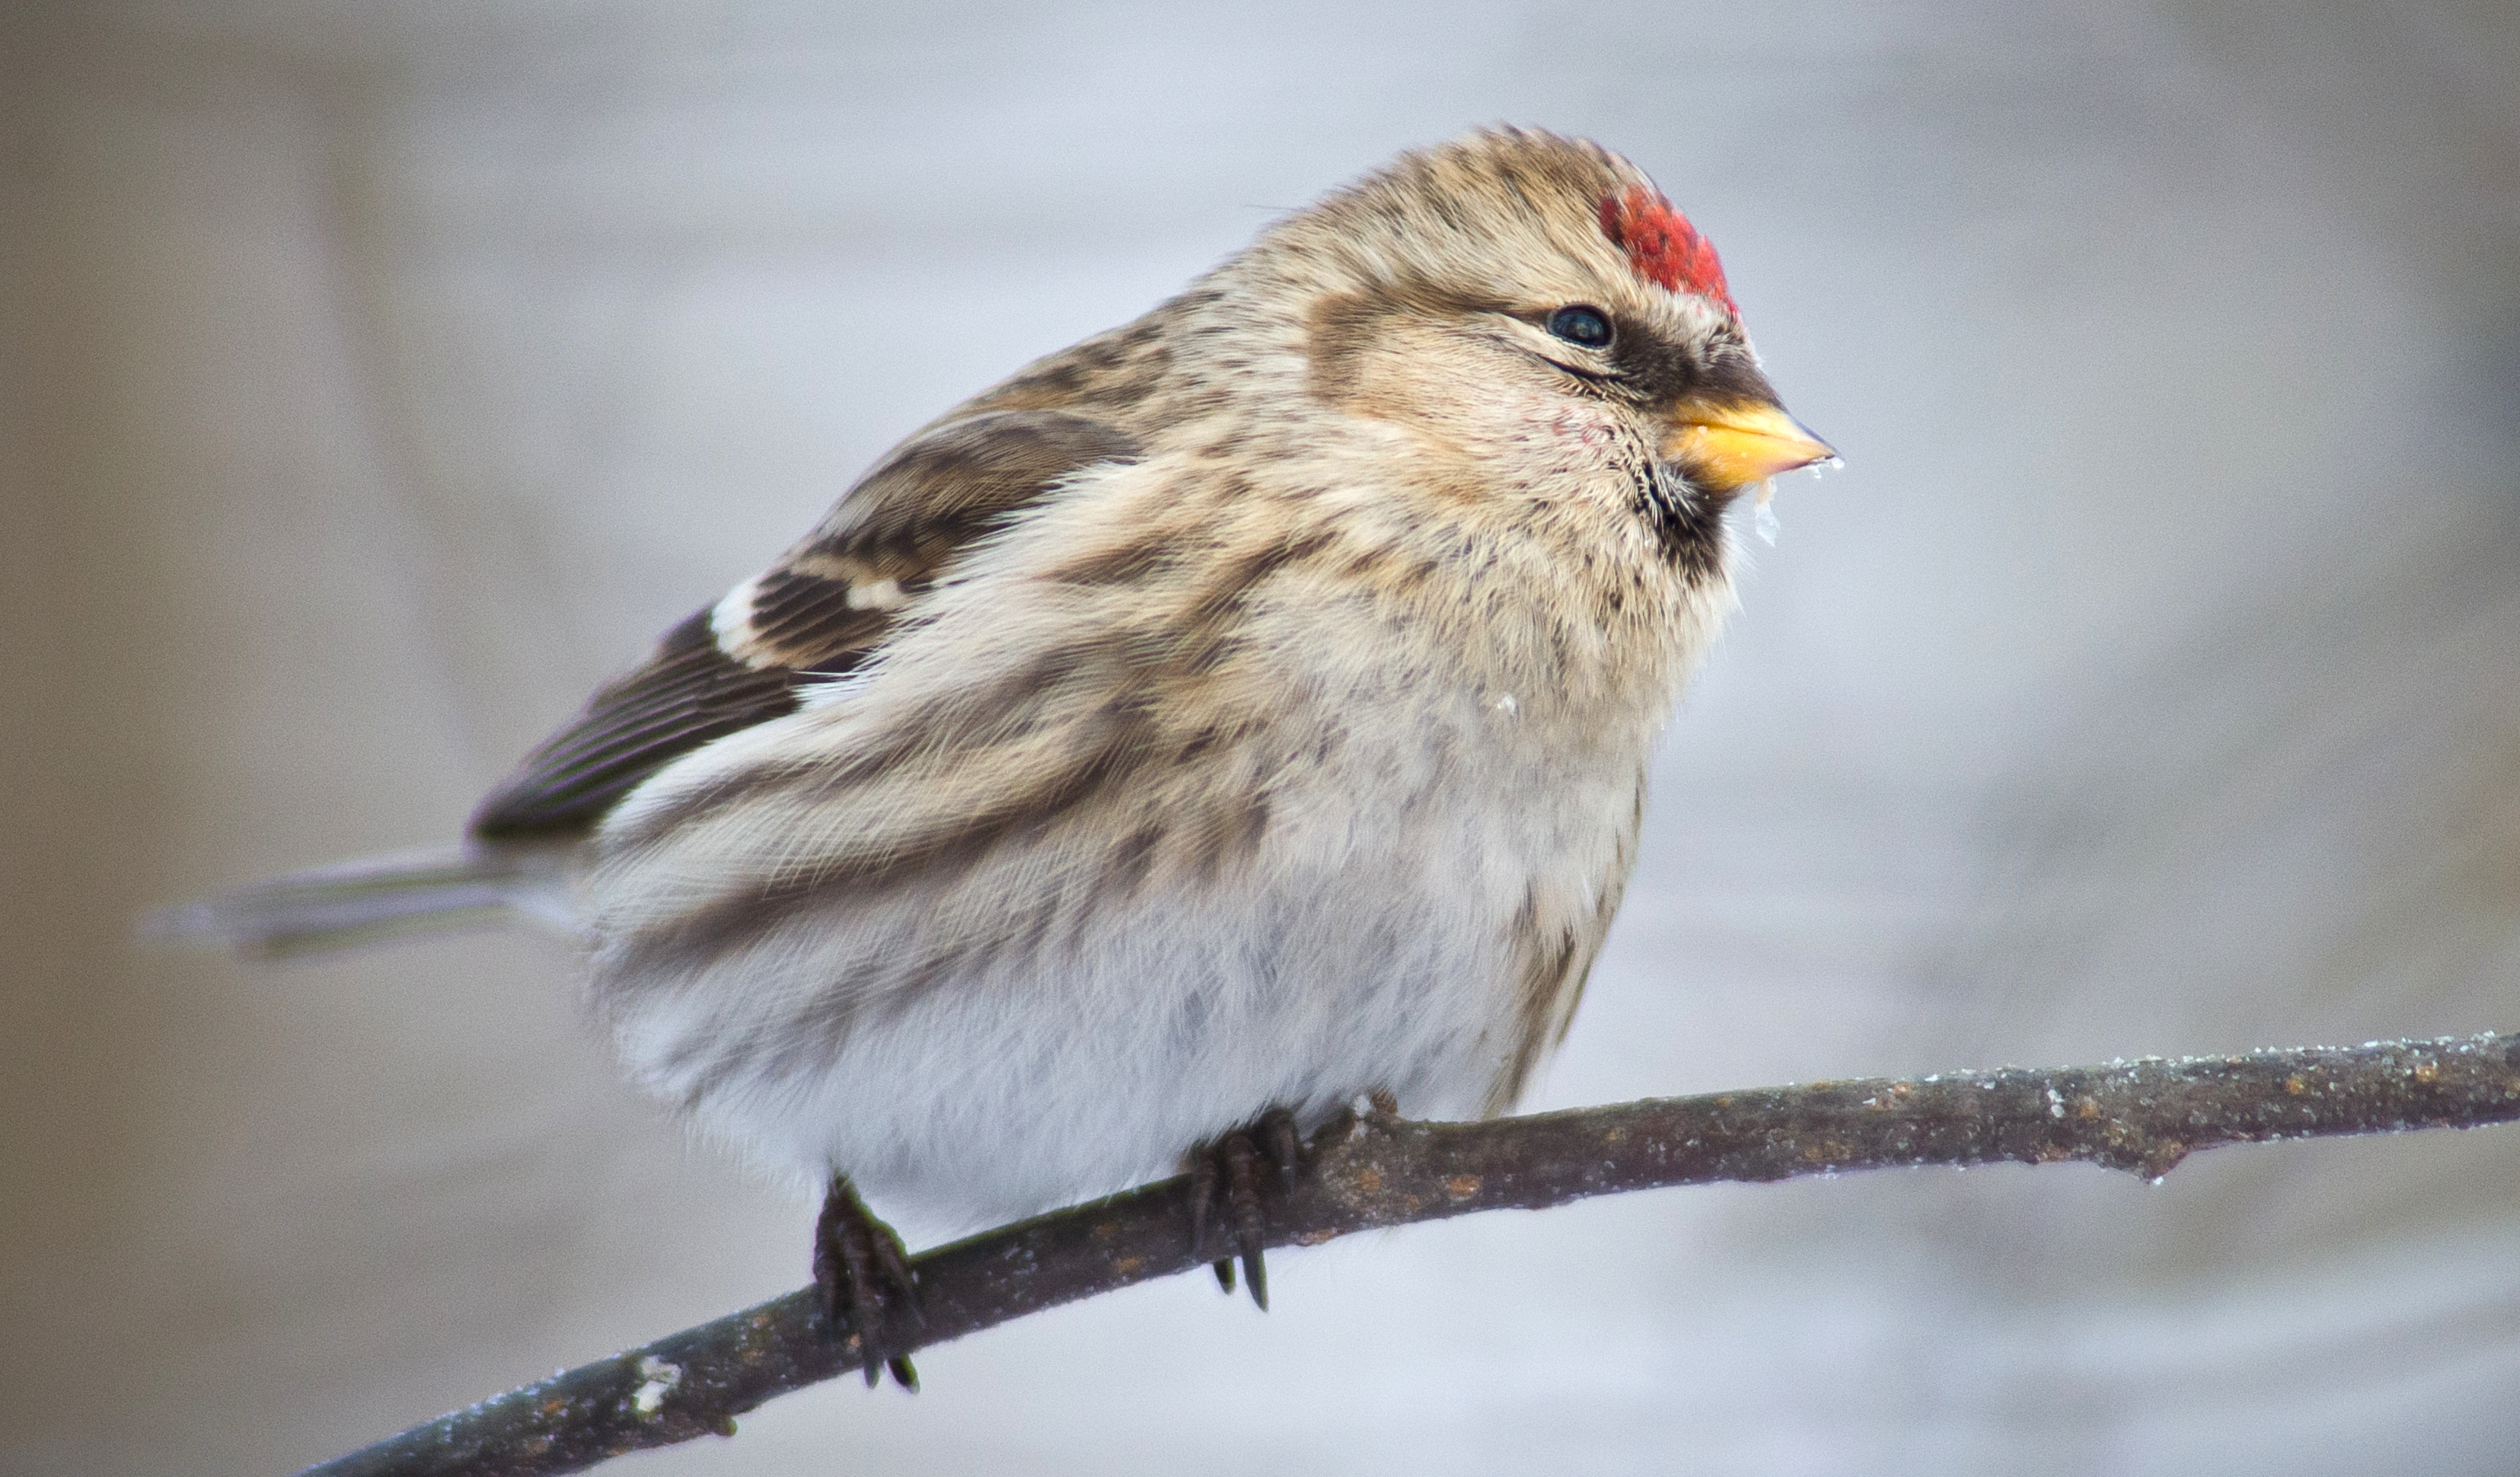
\includegraphics[width=\linewidth]{Acanthis_flammea}
        \caption{A common redpoll (Acanthis Flammea)}
        \label{fig:Acanthis_flammea}
    \end{figure}

\end{center}
\vspace{\baselineskip}

%Students info
\normalsize
\vspace*{\fill}
\begin{flushright}
    Niek R. Scholten (388602)\\
    Bio-Informatics BFV3\\
    Institute of Life Science \& Technology\\
    Hanze University of Applied Sciences\\
    Dave Langers (LADR) \& Bart Barnard (BABA)\\
    \today
\end{flushright}
\newpage

%Blank page
\null
\thispagestyle{empty}
\addtocounter{page}{-1}
\newpage

\begin{center}

%Titles

    \Huge{Predicting bird species from their songs using machine learning}\\
    \vspace{\baselineskip}
    \LARGE{Theme 09 - Introduction Machine Learning}\\
    \vspace{\baselineskip}

\end{center}
\vspace{\baselineskip}

%Students info
\normalsize
\vspace*{\fill}
\begin{flushright}
    Niek R. Scholten (388602)\\
    Bio-Informatics BFV3\\
    Institute of Life Science \& Technology\\
    Hanze University of Applied Sciences\\
    Dave Langers (LADR) \& Bart Barnard (BABA)\\
    \today
\end{flushright}
\newpage

\pagenumbering{roman}
\section*{Abstract}

The complexity and the consistency of birds' songs have long been marveled over.
And they always say ``consistency is key'', which is also true for the models in this project.
All the data that was used follows nice conventions and is perfect for machine learning.
This study aims to find out how well new songs of those same bird species can be classified using a model trained on the original data using machine learning.

\label{sec:abstract}~\addcontentsline{toc}{section}{\nameref{sec:abstract}}
\newpage

\section*{Summary}

Birds' songs can be complex and hard to distinguish by ear, but these songs can be easily transcribed to numeric data which is easily understood by computers.
The goal of this research is to create an easy to run program that can classify new instances of this numeric convention.
Python was used in pre-processing to make sure all data was structured correctly and ready for visualisation.
Weka was used after this to explore possible models for the dataset, the best model was chosen and exported to be used in a Java program.
The wrapper has been successfully built and can classify new instances with a high accuracy.

\label{sec:summ}~\addcontentsline{toc}{section}{\nameref{sec:summ}}
\newpage

\section*{List of Abbreviations}

\textbf{CSV} Comma-separated values

\textbf{STFT} Short-time Fourier transform

\label{sec:abvs}~\addcontentsline{toc}{section}{\nameref{sec:abvs}}

\newpage

{
\setcounter{tocdepth}{2}
\tableofcontents
}
\newpage

\pagenumbering{arabic}

\hypertarget{introduction}{%
\section{Introduction}\label{introduction}}

\hypertarget{purpose}{%
\subsection{Purpose}\label{purpose}}

The wonders of birds' songs can best be experienced in person, but to
accurately predict the species can be difficult. This research aims to
provide an easy way to predict the species of a bird song.

\hypertarget{theory}{%
\subsection{Theory}\label{theory}}

\hypertarget{sound-theory}{%
\subsubsection{Sound theory}\label{sound-theory}}

The provided data has 2 different kinds features; chroma features \&
spectral centroids. These features are calculated on 13 intervals from a
pre-defined random ``window'\,' of a bird's song. There are 12 chroma
features and 1 spectral centroid per interval. So in the end each sample
of a song is converted to 168 numeric data points (13 features * 13
intervals).

\hypertarget{chroma-features}{%
\paragraph{Chroma features}\label{chroma-features}}

capture the melodic characteristics of music, they capture the intensity
of a certain tone at any given time. Each of the tone heights in an
octave fits into a set of chroma features: \{C, C\#, D, D\#, E , F, F\#,
G, G\#, A, A\#, B\}. These features are calculated using STFT's
(Short-time Fourier transform). \[
{\displaystyle {\hat {f}}(\xi )=\left\{{\begin{aligned}&\int _{-\infty }^{\infty }f(x)\ e^{-i2\pi \xi x}\,dx,\ &\xi \geq 0\\&{\hat {f}}^{*}(|\xi |)&\xi <0\\\end{aligned}}\right.,}
\]

\begin{center}
(\label{eq:eq1}1.2.1.1 A Fourier transform, $x$ represents time. [\ref{ref:ref1}])
\end{center}

A STFT uses equation \ref{eq:eq1} on every interval of an audio clip to
generate the chroma features.

\hypertarget{spectral-centroid}{%
\paragraph{Spectral centroid}\label{spectral-centroid}}

is described as the center of mass of a spectrum. It is also known as
the ``brightness'\,' or timbre of sound. It is also calculated using a
Fourier transform \ref{eq:eq1} with the magnitude used as weights.

\[
{\displaystyle \mathrm {Centroid} ={\frac {\sum _{n=0}^{N-1}f(n)x(n)}{\sum _{n=0}^{N-1}x(n)}}}
\]

\begin{center}
(\label{eq:eq2}1.2.1.2 The formula for calculating the centroid, $x(n)$ represents magnitude. [\ref{ref:ref2}])
\end{center}

\hypertarget{algorithm-theory}{%
\subsubsection{Algorithm theory}\label{algorithm-theory}}

The algorithm used for this research is called a random forest. It
combines regular decision trees with bagging to create a ``forest'\,' of
randomized decision trees. Regular decision trees are very prone to
overfitting (matching the orignal data too much) the deeper they get,
increasing irregularity. The reason random forest is so powerful is that
it averages multiple decision trees to create a model that's not as
biased as regular decision trees and less irregular.

\hypertarget{bagging}{%
\paragraph{Bagging}\label{bagging}}

splits up a data set and trains the model on these splits, only to
recombine them later on. This greatly reduces overfitting and increases
variance.

\hypertarget{decision-trees}{%
\paragraph{Decision trees}\label{decision-trees}}

create leaves that represent the class labels and branches that
represent decision paths. A new instance can then be entered into it, so
it will end at one of these leaves in accordance to its values. \newpage

\hypertarget{materials-methods}{%
\section{Materials \& Methods}\label{materials-methods}}

The dataset contains converted data from bird song samples. The
datapoints contain information about the intensity of certain tones in
these samples. The CSV data was supplied by
\href{https://www.kaggle.com/datasets/fleanend/birds-songs-numeric-dataset}{Edoardo
Ferrante on Kaggle}. This data was created using the Librosa package for
Python. Librosa outputs the intensity of a certain tone at different
time intervals from the provided sound file. There is a Python script
available from the author that explains how the data was transformed
from sound files to numeric data points, but this script has a specific
shortcoming that will be explained later.

\hypertarget{materials}{%
\subsection{Materials}\label{materials}}

Several pieces of software were used over the course of this research,
from packages to programs. The data was supplied by
\href{https://www.kaggle.com/datasets/fleanend/birds-songs-numeric-dataset}{Edoardo
Ferrante on Kaggle} and contains CSV (comma-seperated values) files for
both training and testing.

\hypertarget{programs}{%
\subsubsection{Programs}\label{programs}}

\begin{longtable}[]{@{}lll@{}}
\toprule
\textbf{Software} & \textbf{Package} & \textbf{Version} \\
\midrule
\endhead
R & & 4.2.1 \\
& Dict & 0.1.0 \\
& dplyr & 1.0.9 \\
& ggbiplot2 & 0.55 \\
& ggplot2 & 3.3.6 \\
& ggpubr & 0.4.0 \\
& knitr & 1.40 \\
& plyr & 1.8.7 \\
& RWeka & 0.4-44 \\
& scales & 1.2.1 \\
Python & & 3.10 \\
& librosa & 0.9.2 \\
& matplotlib & 3.5.3 \\
& numpy & 1.23.3 \\
& pandas & 1.4.4 \\
Weka & & 3.8.6 \\
& wekaDeeplearning4j & 1.7.2 \\
Java & openJDK17 & 17.0.4 \\
Gradle & & 7.4 \\
& weka-stable & 3.8.6 \\
\bottomrule
\end{longtable}

\begin{center}
Table 1: Programs and versions \label{tab:tab1}
\end{center}

The data consists of multiple iterations of the original CSV files. A
metadata file is also included as to give some extra context to the
source of the audio files.

\newpage

\hypertarget{methods}{%
\subsection{Methods}\label{methods}}

Pre-processing and model training are the most intense operations
performed in this research. There was also a bit of light data
exploration which is contained within the log.

\hypertarget{data-pre-processing}{%
\subsubsection{Data Pre-Processing}\label{data-pre-processing}}

First let's have a look at how Librosa normally outputs the chromogram
data:

\begin{longtable}[]{@{}
  >{\raggedright\arraybackslash}p{(\columnwidth - 14\tabcolsep) * \real{0.1923}}
  >{\raggedright\arraybackslash}p{(\columnwidth - 14\tabcolsep) * \real{0.1154}}
  >{\raggedright\arraybackslash}p{(\columnwidth - 14\tabcolsep) * \real{0.1154}}
  >{\raggedright\arraybackslash}p{(\columnwidth - 14\tabcolsep) * \real{0.1154}}
  >{\raggedright\arraybackslash}p{(\columnwidth - 14\tabcolsep) * \real{0.1154}}
  >{\raggedright\arraybackslash}p{(\columnwidth - 14\tabcolsep) * \real{0.1154}}
  >{\raggedright\arraybackslash}p{(\columnwidth - 14\tabcolsep) * \real{0.1154}}
  >{\raggedright\arraybackslash}p{(\columnwidth - 14\tabcolsep) * \real{0.1154}}@{}}
\toprule
\begin{minipage}[b]{\linewidth}\raggedright
\end{minipage} & \begin{minipage}[b]{\linewidth}\raggedright
0
\end{minipage} & \begin{minipage}[b]{\linewidth}\raggedright
1
\end{minipage} & \begin{minipage}[b]{\linewidth}\raggedright
2
\end{minipage} & \begin{minipage}[b]{\linewidth}\raggedright
3
\end{minipage} & \begin{minipage}[b]{\linewidth}\raggedright
4
\end{minipage} & \begin{minipage}[b]{\linewidth}\raggedright
5
\end{minipage} & \begin{minipage}[b]{\linewidth}\raggedright
6
\end{minipage} \\
\midrule
\endhead
chromogram\_0 & 0.68661 & 0.67378 & 0.65758 & 0.66149 & 0.68533 &
0.72239 & 0.76395 \\
chromogram\_1 & 0.91368 & 0.88148 & 0.85024 & 0.82476 & 0.82282 &
0.83024 & 0.83908 \\
chromogram\_2 & 0.98221 & 0.97060 & 0.95834 & 0.94729 & 0.94785 &
0.95189 & 0.95408 \\
chromogram\_3 & 1.00000 & 1.00000 & 1.00000 & 1.00000 & 1.00000 &
1.00000 & 1.00000 \\
chromogram\_4 & 0.96223 & 0.95790 & 0.95436 & 0.95403 & 0.94404 &
0.93285 & 0.91552 \\
chromogram\_5 & 0.92098 & 0.89960 & 0.88007 & 0.86290 & 0.84262 &
0.82280 & 0.80381 \\
chromogram\_6 & 0.87591 & 0.85544 & 0.83320 & 0.80870 & 0.78241 &
0.75819 & 0.73456 \\
chromogram\_7 & 0.79397 & 0.79418 & 0.79848 & 0.80535 & 0.80741 &
0.80750 & 0.80913 \\
chromogram\_8 & 0.62856 & 0.64859 & 0.68255 & 0.72441 & 0.76565 &
0.80078 & 0.82178 \\
chromogram\_9 & 0.41881 & 0.41914 & 0.44003 & 0.48525 & 0.54615 &
0.61608 & 0.68581 \\
chromogram\_10 & 0.36895 & 0.38299 & 0.40678 & 0.43114 & 0.45138 &
0.47237 & 0.52333 \\
chromogram\_11 & 0.33855 & 0.34676 & 0.35929 & 0.37378 & 0.38602 &
0.39931 & 0.42756 \\
\bottomrule
\end{longtable}

\begin{center}
Table 2: Librosa output data \label{tab:tab2}
\end{center}

As you can see, the output is a neat array containing the values of 12
different tones at different time intervals. This data is sorted and can
be read by Librosa.

Now onto the issue; the provided dataset contains this data in a stacked
order, so each sample only takes up one row. This is a good idea, but
due to sorting by alphabetical order the original order is lost. The
order is important because we are working with data over time. This is
not a problem if the trained model is only used on the provided test
data, but we want the trained model to work in as many situations as
possible.

\newpage

Here is a look at the provided data:

\begin{longtable}[]{@{}
  >{\raggedright\arraybackslash}p{(\columnwidth - 8\tabcolsep) * \real{0.0581}}
  >{\raggedright\arraybackslash}p{(\columnwidth - 8\tabcolsep) * \real{0.2442}}
  >{\raggedright\arraybackslash}p{(\columnwidth - 8\tabcolsep) * \real{0.2442}}
  >{\raggedright\arraybackslash}p{(\columnwidth - 8\tabcolsep) * \real{0.2209}}
  >{\raggedright\arraybackslash}p{(\columnwidth - 8\tabcolsep) * \real{0.2326}}@{}}
\toprule
\begin{minipage}[b]{\linewidth}\raggedright
id
\end{minipage} & \begin{minipage}[b]{\linewidth}\raggedright
chromogram\_0\_0
\end{minipage} & \begin{minipage}[b]{\linewidth}\raggedright
chromogram\_0\_1
\end{minipage} & \begin{minipage}[b]{\linewidth}\raggedright
chromogram\_0\_10
\end{minipage} & \begin{minipage}[b]{\linewidth}\raggedright
chromogram\_0\_11
\end{minipage} \\
\midrule
\endhead
0 & 0.997943662321316 & 0.832392210770135 & 0.7653861625931 &
0.70427464132375 \\
1 & 0.996254885931866 & 0.839119599044146 & 0.760416790506312 &
0.705141765139875 \\
2 & 0.970810156116343 & 0.823539694937237 & 0.759508104372184 &
0.709057883677716 \\
3 & 1 & 0.855558393364941 & 0.752038009313116 & 0.710976936190937 \\
4 & 1 & 0.884304523555434 & 0.741884532311754 & 0.714775207828629 \\
5 & 0.971867873978603 & 0.824311712155432 & 0.755293860709407 &
0.71448132195049 \\
6 & 1 & 0.835499361583387 & 0.751917158063063 & 0.717361992854453 \\
7 & 0.978929855885584 & 0.827216718543843 & 0.751072631712318 &
0.718400862681119 \\
8 & 1 & 0.895339720206626 & 0.733409813021178 & 0.722747412968086 \\
9 & 0.967651828343747 & 0.823697857901917 & 0.746005680687241 &
0.721194823494439 \\
10 & 0.993699774531599 & 0.847257121555946 & 0.734368883301346 &
0.726420069139032 \\
11 & 0.00947350497274455 & 0.00699383738737368 & 0.372026644035831 &
0.0516494292032762 \\
12 & 0.00982270123521504 & 0.00712337798131429 & 0.371129653847745 &
0.051631441504244 \\
\bottomrule
\end{longtable}

\begin{center}
Table 3: Provided data \label{tab:tab3}
\end{center}

Each row contains a stack of chromogram data in a non-sequential order.
The end of the array also contains the species of the corresponding bird
and some spectral centroid data.

\begin{figure}
    \centering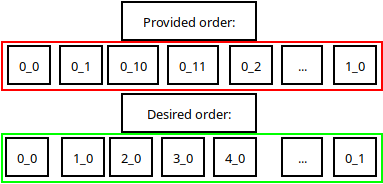
\includegraphics[width=\linewidth]{../figures/data_flow.png}
    \caption{Comparison of the data order}
    \label{fig:fig2}
\end{figure}

Figure \ref{fig:fig2} shows a comparison of the order of provided data
and the ideal order the data should be sorted in. A Python script was
used to re-order the data into this format.

Data exploration was not a big part of this research, the data was
fairly straightforward after this initial processing. Some exploration
was done to look at differences between the species, this is further
fleshed out in the results.

While exploring the data, all instances were exported to arff files
using the RWeka package. In Weka these were subsequently altered so the
class labels were nominal values and placed in the last column. An extra
test data set was also created with all of its instances randomized, so
there was no bias to the order.

\newpage

\hypertarget{model-training}{%
\subsubsection{Model training}\label{model-training}}

To create a usable model in Weka, a lot of algorithms were tested for
efficiency. Namely:

\begin{longtable}[]{@{}l@{}}
\toprule
Algorithm \\
\midrule
\endhead
ZeroR \\
OneR \\
NaiveBayes \\
Sequential minimal optimization \\
SimpleLogistic \\
IBk \\
J48 Tree \\
RandomForest \\
wekaDeeplearning4j \\
\bottomrule
\end{longtable}

\begin{center}
Table 4: Tested algorithms \label{tab:tab4}
\end{center}

The option of wekaDeeplearning4j was explored, but due to the difficult
nature to set up and lackluster performance compared to cheaper
algorithms it was not explored further.

All models were trained on the train dataset using 10-fold
cross-validation with varying results. The random forest model file was
exported for later use in the wrapper.

\hypertarget{wrapper-creation}{%
\subsubsection{Wrapper creation}\label{wrapper-creation}}

The finalized wrapper was built using Gradle and the weka-stable package
for Java. The aforementioned model file containing the trained random
forest model is incorporated into the jar file and shipped with the
program. It was tested on the unlabeled test data set and validated
afterwards using the correct labels.

\newpage

\hypertarget{results}{%
\section{Results}\label{results}}

The results of this research come in 2 sections, exploration and model
performance. The exploration section contains some results of the
exploratory data analysis along with figures to sketch an idea of the
data that was used. The section on model performance contains detailed
information about the model that was chosen as final classifier.

\hypertarget{exploration}{%
\subsection{Exploration}\label{exploration}}

\begin{figure}
\centering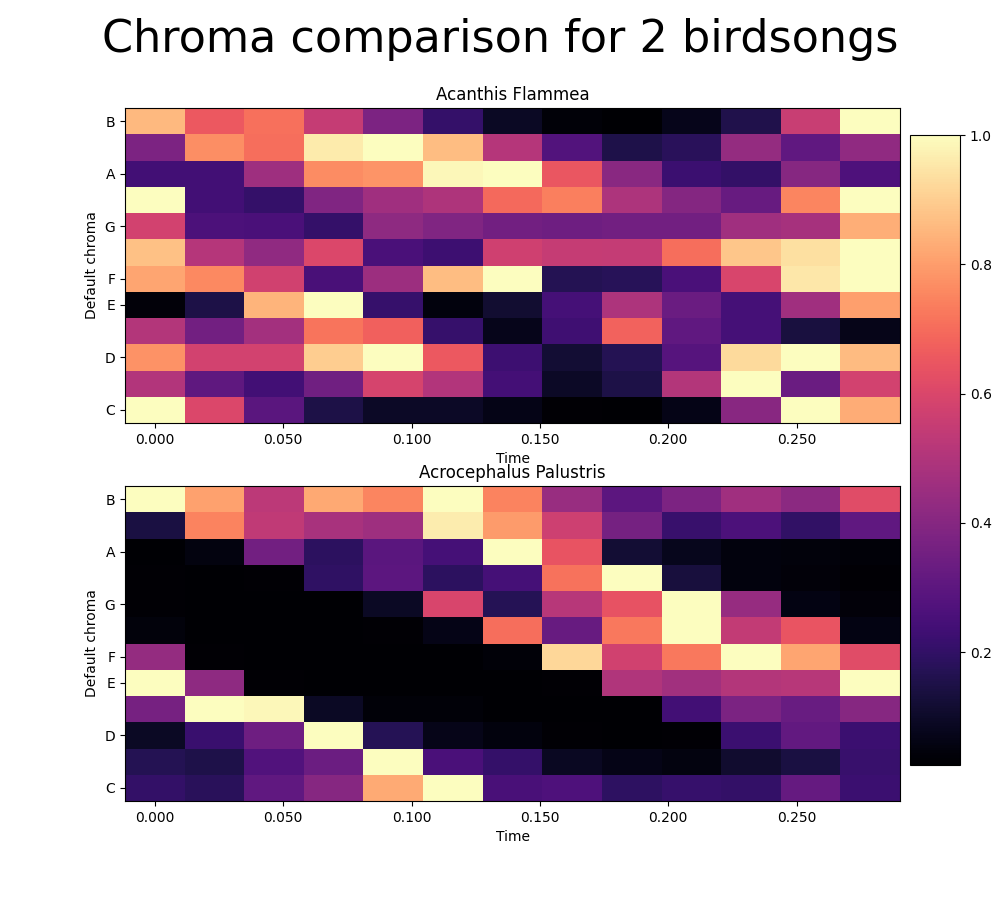
\includegraphics[width=\linewidth]{../figures/chroma_comparison.png}
\caption{Chroma signature comparison for 2 fragments of different bird-species songs}
\label{fig:fig3}
\end{figure}

Figure \ref{fig:fig3} shows the first result of the data exploration.
There is a clear difference in signature between the two species. This
difference can be explored further by analyzing one tone at the time.

\newpage

\begin{figure}
\centering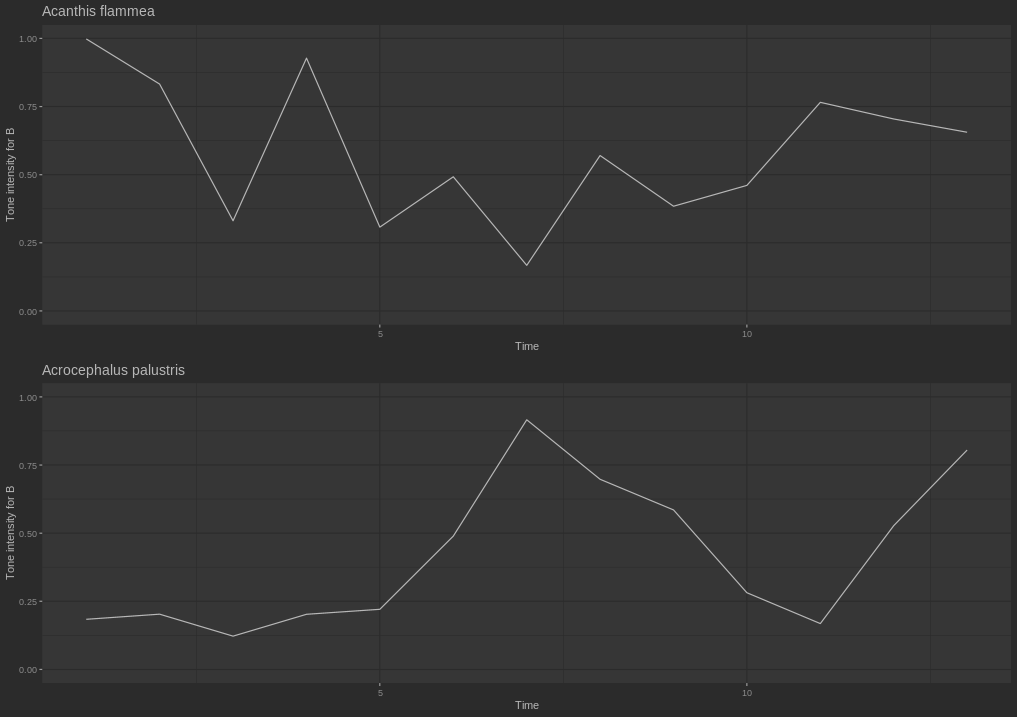
\includegraphics[width=\linewidth]{../figures/B_comparison.png}
\caption{Tone intensity comparison at tone B for 2 fragments of different bird-species songs}
\label{fig:fig4}
\end{figure}

Figure \ref{fig:fig4} also shows a clear difference in tone intensity
over the duration of the sound fragment. Tone B was chosen as an
example, but multiple tones exhibit this behaviour as seen in Figure 2.

\newpage

\begin{figure}
\centering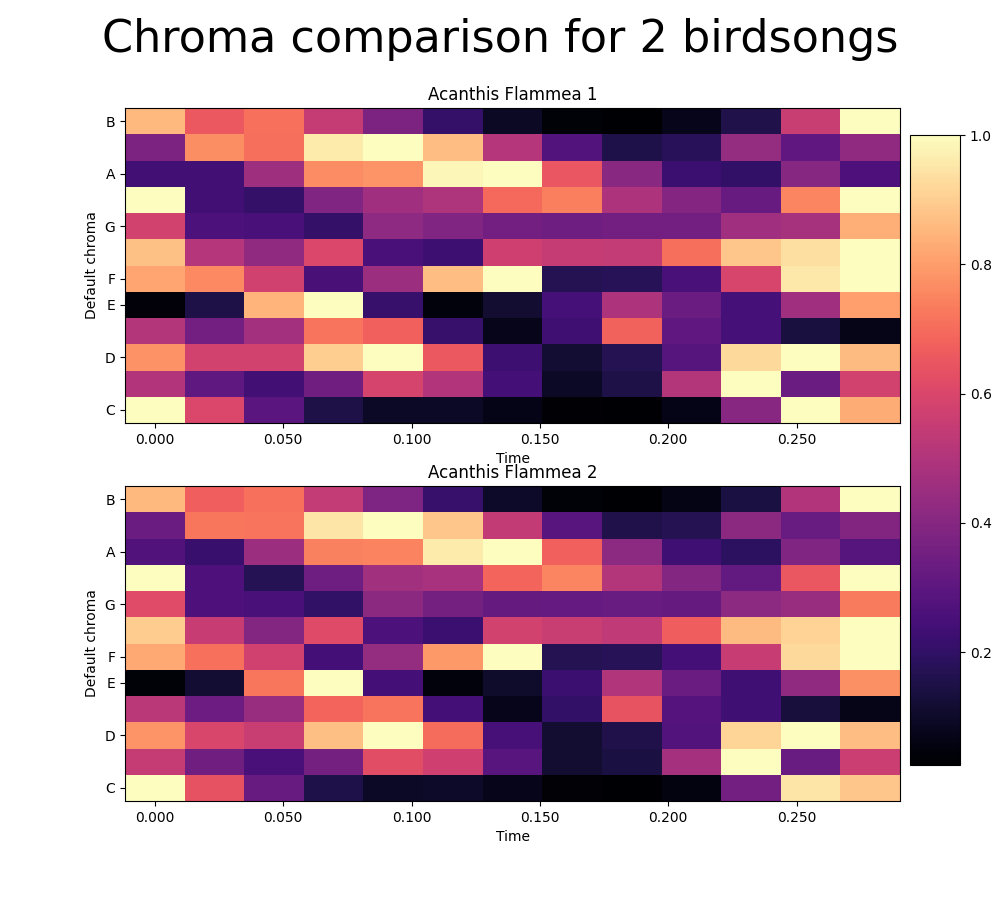
\includegraphics[width=\linewidth]{../figures/chroma_comparison_same.png}
\caption{Chroma signature comparison for 2 fragments of the same bird-species songs}
\label{fig:fig5}
\end{figure}

Lastly, figure \ref{fig:fig5} shows the signature comparison of 2 bird
songs of the same species. These signatures look alike, but there are
subtle differences to be seen.

\newpage

\hypertarget{model-performance}{%
\subsection{Model performance}\label{model-performance}}

As mentioned in previous chapters, the random forest classifier is the
best one for this specific use case. It was chosen by evaluating
different models using the Weka experimenter. Pinning these models
against each other yielded the following results:

\begin{longtable}[]{@{}ll@{}}
\toprule
Algorithm & \% correct \\
\midrule
\endhead
ZeroR & 1.14 \\
OneR & 52.45 \\
NaiveBayes & 92.12 \\
Sequential minimal optimization & 98.06 \\
SimpleLogistic & 98.02 \\
IBk & 98.13 \\
J48 Tree & 93.40 \\
RandomForest & 98.55 \\
\bottomrule
\end{longtable}

\begin{center}
Table 5: Tested algorithms and their performance \label{tab:tab5}
\end{center}

As seen above, the performarce of the random forest is almost matched in
a few cases, but with some tweaks a \% correct score of 98.8632 \% was
achieved. Here are the parameters used to achieve this result:

\begin{verbatim}
weka.classifiers.trees.RandomForest -- -P 100 -I 110 -num-slots 12 -K 0 -M 1.0 -V 0.001 -S 1
\end{verbatim}

Another upside of the random forest classifier is its speed, it is able
to work in parallel and increase performance linearly. Other models take
a lot of time to train and test using cross validation.

OneR also scores pretty high, indicating that one label can be enough to
correctly classify most of the data. In this case the spectral centroids
hold a lot of information, as this is what OneR uses as label. If this
specific spectral centroid is removed from the dataset, the performance
doesn't drop that much since it will use another spectral centroid.
However, if all spectral centroids are removed, OneR's performance falls
to 30\%. This indicates that spectral centroids hold a lot of
information about the birds' species.

Because the train and test set are of differing sizes, they are
incompatible. Therefore, the model has to be passed through
\texttt{weka.classifiers.misc.InputMappedClassifier} to be able to test
on the test set. This is also incorporated in the Java wrapper.

\newpage

\begin{figure}
\centering
\includegraphics{/home/nieks/IdeaProjects/Thema9-Praktijkopdracht/final_report/final_report_files/figure-latex/ROC-1.pdf}
\caption{\label{fig:fig6}ROC Curve of Acanthis Flammea}
\end{figure}

The figure above shows the ROC Curve for Acanthis Flammea, the model is
able to classify all instances of the test set perfectly. The training
set is balanced, containing 20 samples of each species, this attributes
to the great results of this model.

\newpage

\hypertarget{conclusion}{%
\section{Conclusion}\label{conclusion}}

Concluding from the data, it seems there is a high probability of
success when training a machine learning model on this data. The
signatures of the same species align with each other nicely and the
signatures of other species are different enough to be separated.
Although the signatures of the same species look alike, there are subtle
differences in the intensity. We can also conclude from this that birds
of the same species sing the same songs.

And from the model creation we can conclude that this was an absolute
success. It can predict new instances with an extremely high accuracy
and few incorrectly classified instanced. The balance between high
accuracy and overfitting is just right, exceeding expectations.

\hypertarget{discussion}{%
\section{Discussion}\label{discussion}}

The model is not perfect, if it was it would have achieved perfect
scores over the entire test set. A randomized train set could be created
by merging the current train and test sets to form one large data set.
This could potentially increase the performance even more as there is
more information variance available, but the current model already
achieves high performance with just 20 entries of every species.

The model could also be expanded to work on longer fragments of songs or
more bird species altogether. \newpage

\hypertarget{references}{%
\section{References}\label{references}}

\begin{enumerate}
\def\labelenumi{\arabic{enumi}.}
\tightlist
\item
  Chroma Feature Extraction, 2019 Ayush Kumar Shah: ResearchGate
  330796993 \label{ref:ref1}
\item
  Brain Seizure Detection and Classification Using EEG Signals, 2022
  Varsha K.Harpale: ScienceDirect B978-0-32-391120-7.00008-6
  \label{ref:ref2}
\end{enumerate}

\end{document}
